\section{证据二：隐藏状态轨迹、固定点、周期与推理阶段}
\label{sec:mechanistic-analysis}

本章的核心判断是：多跳性能提升只能说明循环深度可能有用，机制分析才开始回答“模型内部是否形成了有结构的递归过程”。视频给出的证据链是：追踪隐藏状态，用主成分分析（Principal Component Analysis, PCA）投影到低维空间，观察固定点与周期轨迹，再检查注意力行为和早期、中期、后期递归阶段是否出现稳定分工。

\begin{importantbox}{本章主张}
权重共享不等于每一步执行同样的功能。输入到共享块的隐藏状态每轮都不同，同一个函数会在不同递归阶段呈现不同作用：早期形成粗表示，中期整合关系，后期稳定并收敛到答案。
\end{importantbox}

\subsection{为什么性能证据还不够}

视频在 00:08:31--00:08:49 明确提出了一个必要怀疑：即使模型多跳表现更好，也不能只凭结果断言它“真的在推理”。一个模型可能因为数据分布、任务模板、训练捷径而表现提升；要建立更强判断，需要看递归过程内部是否有可观察结构。

这里的第一性原理很直接：若循环模型只是把隐藏状态随机扰动几次，性能偶然提升的解释就很脆弱；若隐藏状态沿着稳定轨迹移动，且注意力行为也随之稳定，读者才有理由相信递归步骤在执行某种一致的计算。机制证据并不会把模型彻底解释清楚，它能排除一部分“只是乱动”的解释。

\subsection{PCA：把高维递归轨迹压到可观察平面}

隐藏状态通常有几千甚至上万维，人眼无法直接观察。PCA 的作用是找出激活变化最大的几个方向，把高维状态投影到二维或三维平面。这样读者可以看到递归轨迹是向某个区域收敛、围绕某个轨道运动，还是快速散开。

先用白话解释下面的公式：PCA 会从一批隐藏状态里估计平均状态 \(\mu\)，再取最能解释变化的主方向 \(W_k\)。每个高维状态 \(h_t\) 被减去均值后投影到这些主方向上，得到低维坐标 \(z_t\)。

\[
z_t=W_k^\top(h_t-\mu),\qquad k\in\{2,3\}
\]

符号说明：
\begin{itemize}
  \item \(h_t\)：第 \(t\) 次递归后的高维隐藏状态。
  \item \(\mu\)：用于居中的平均隐藏状态。
  \item \(W_k\)：前 \(k\) 个主成分方向组成的矩阵。
  \item \(z_t\)：低维投影坐标，用于画出递归轨迹。
  \item \(k\)：投影维度，常取 \(2\) 或 \(3\)，便于可视化。
\end{itemize}

\begin{knowledgebox}{PCA 的作用边界}
PCA 像给高维房间装一盏投影灯：它能把主要运动方向投到墙上，让人看见轨迹形状。代价也很清楚，墙上的影子会丢掉一部分维度信息，所以 PCA 图适合提示结构，不能单独充当完整证明。
\end{knowledgebox}

\subsection{固定点与周期：递归过程趋向稳定结构}

视频在 00:09:20--00:09:43 说明，机制分析观察到循环模型在潜在空间中趋向稳定轨迹：一些情况像固定点，表示表征逐渐稳定；另一些情况呈现周期轨迹，隐藏状态在重复块中访问一致状态。这说明内部状态没有不可预测地快速坍缩，也没有无界漂移。

固定点表达的是“更新后几乎仍在原处”。在推理语境里，它可以理解为模型已经把相关信息整合到一个稳定表示中，继续递归带来的变化变小。

\[
h^\star \approx F_\theta(h^\star,x)
\]

符号说明：
\begin{itemize}
  \item \(h^\star\)：稳定隐藏状态或近似收敛点。
  \item \(F_\theta\)：共享递归模块。
  \item \(x\)：输入或上下文。
  \item \(\approx\)：近似相等，表示实际观测中存在小幅更新。
\end{itemize}

周期轨迹表达的是“隔若干轮回到相似位置”。它不代表模型没有进展，可能代表系统在几个互补状态之间有规律切换，例如反复在候选关系和答案表示之间调整。

\[
h_{t+p}\approx h_t,\qquad p\ge 2
\]

符号说明：
\begin{itemize}
  \item \(h_t\)：第 \(t\) 次递归后的状态。
  \item \(h_{t+p}\)：经过 \(p\) 轮后的状态。
  \item \(p\)：周期长度。
  \item \(\approx\)：表示两个状态在低维投影或相似性度量上接近。
\end{itemize}

\begin{figure}[htbp]
  \centering
  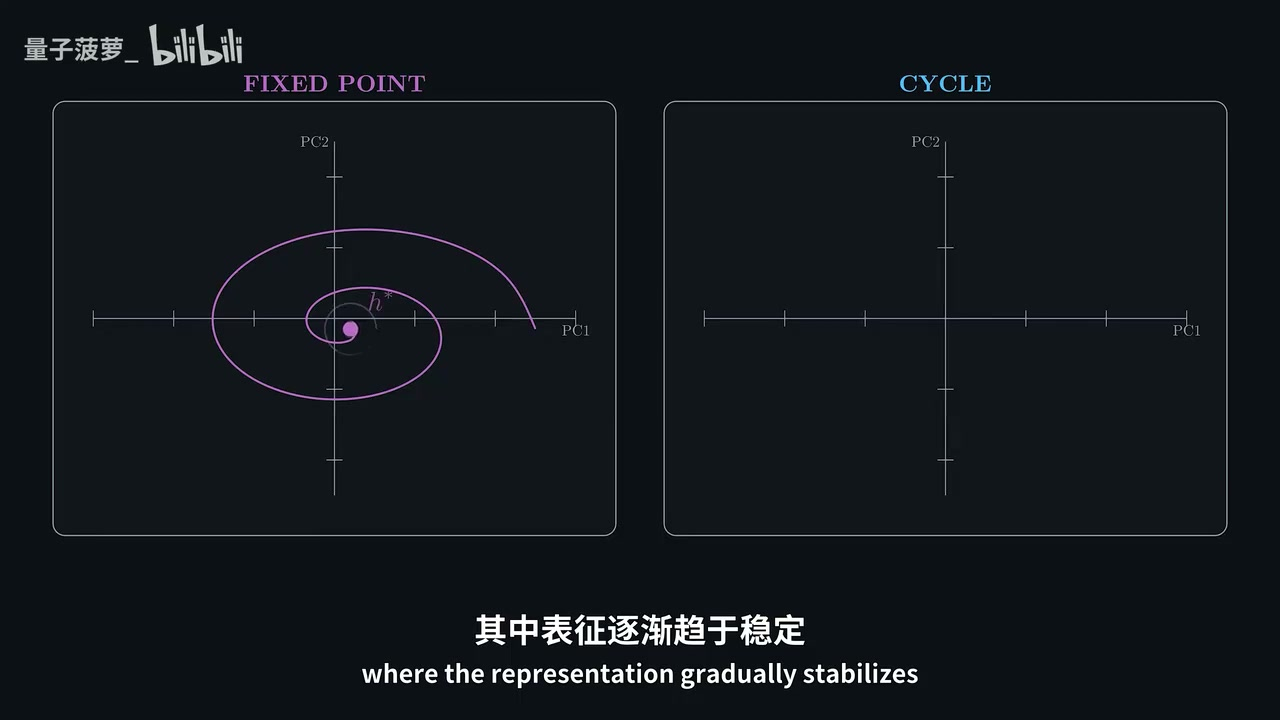
\includegraphics[width=0.82\linewidth,height=0.36\textheight,keepaspectratio]{figures/fig_09_fixed_point_cycle.jpg}
  \caption{PCA 视角下的固定点与周期轨迹：前者显示状态逐步稳定，后者显示状态在一致区域之间有规律往复。\protect\footnotemark}
  \label{fig:pca-fixed-point-cycle}
\end{figure}
\footnotetext{视频画面时间区间：00:09:20--00:09:37。}

\subsection{注意力稳定：状态稳定还要对应计算稳定}

只看激活轨迹仍然不够。隐藏状态稳定可能只是数值上变得平滑，未必意味着模型正在执行一致计算。视频在 00:09:43--00:10:00 补了第二层证据：当隐藏状态接近固定点或周期轨迹时，注意力头（attention head）的行为也趋于稳定；这意味着块内部执行的计算也更一致。

这个点很关键。attention 决定了 token 之间如何交换信息。若隐藏状态轨迹趋稳，同时 attention 模式也趋稳，那么递归过程更像一个逐步收敛的计算程序；若两者分离，PCA 图就可能只是漂亮的几何图案。讲义需要把这一层边界讲清楚：机制证据的强度来自多种观测相互支持，而非单张 PCA 图。

\begin{warningbox}{机制证据边界}
PCA 图不能直接证明“模型学会了人类可解释的推理算法”。它能显示轨迹形状，注意力分析能补充计算行为是否稳定；二者合在一起，才构成比性能曲线更强的机制线索。
\end{warningbox}

\subsection{早期、中期、后期：共享块如何形成阶段化功能}

视频在 00:10:02--00:11:00 给出了本章最有教学价值的观察：同一共享块在递归过程的不同阶段承担不同角色。早期递归构建问题的粗略表示，收集并组织相关信息，更新幅度更大也更具探索性；中期递归开始整合信息并传递关系，更新更结构化；后期递归主要稳定表示并收敛到最终答案。

这件事听起来反直觉，因为共享权重意味着每轮调用的是同一个函数。关键在于函数的输入已经变了。可把共享块想成同一位编辑：第一遍拿到的是混乱草稿，所以任务是搭框架；第二遍看到的是已有结构的稿件，所以任务变成补关系；最后一遍面对接近完成的稿件，任务转为收敛和校正。同一位编辑，面对不同阶段的文本，会做出不同动作。

\begin{figure}[htbp]
  \centering
  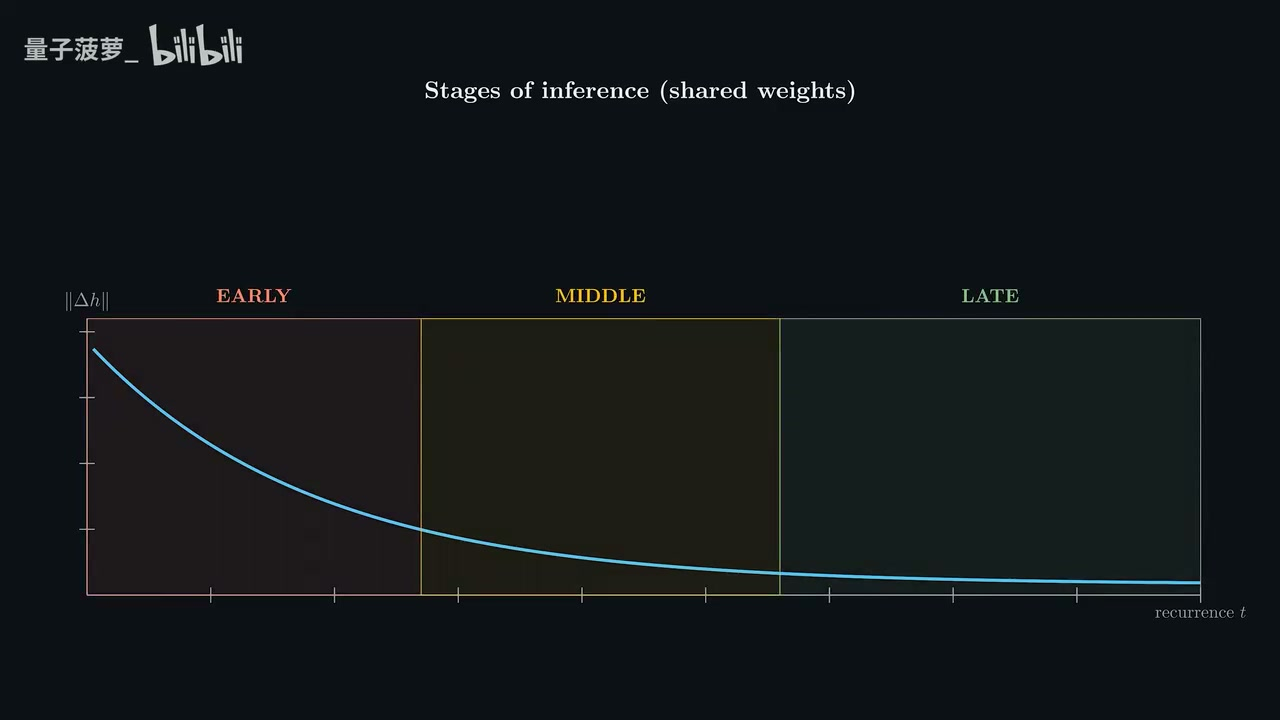
\includegraphics[width=0.82\linewidth,height=0.36\textheight,keepaspectratio]{figures/fig_10_stages_of_inference.jpg}
  \caption{共享权重下的推理阶段：早期更新幅度大，中期逐步结构化，后期趋于稳定和收敛。\protect\footnotemark}
  \label{fig:stages-of-inference}
\end{figure}
\footnotetext{视频画面时间区间：00:10:02--00:10:45。}

可以用一个简单的更新差分表达阶段变化。它先说明每一轮状态变化有多大，再把“早期大、中期结构化、后期变小”落到数学对象上。

\[
\Delta_t=h_{t+1}-h_t,\qquad \lVert \Delta_{\mathrm{early}}\rVert>\lVert \Delta_{\mathrm{late}}\rVert
\]

符号说明：
\begin{itemize}
  \item \(\Delta_t\)：第 \(t\) 次递归带来的状态变化。
  \item \(h_t\)：第 \(t\) 次递归后的隐藏状态。
  \item \(h_{t+1}\)：下一轮隐藏状态。
  \item \(\lVert \Delta_{\mathrm{early}}\rVert\)：早期递归更新幅度。
  \item \(\lVert \Delta_{\mathrm{late}}\rVert\)：后期递归更新幅度。
\end{itemize}

这个式子不声称所有模型都必须满足严格单调下降。它只是在讲义中表达视频所说的阶段化直觉：早期更像探索，中期更像关系整合，后期更像稳定答案。

\subsection{本章小结}

本章把“递归可能增强推理”的说法推进到机制层面。读者应带走四点：第一，性能提升需要内部轨迹证据支持；第二，PCA 能把高维状态投影成可观察轨迹，也会丢失信息；第三，固定点、周期和注意力稳定共同提示递归过程具有结构；第四，共享权重仍可形成阶段化功能，因为每一轮输入到共享块的状态已经不同。下一章将沿着这个逻辑追问计算效率：既然所有 token 固定递归会浪费计算，MoR 如何让不同 token 使用不同递归深度。
